\documentclass[10pt,conference,compsocconf]{IEEEtran}
\usepackage{graphicx}
\usepackage{amsmath}
\usepackage{hyperref}
\usepackage{cite}

\title{PCA and autoencoders: a comparison on image denoising}
\author{
  \begin{tabular}{ccc}
    Luca Bulgarelli & Alessandro Ferrera & Tommaso Fioratti \\
    \texttt{luca.bulgarelli@epfl.ch} & 
    \texttt{alessandro.ferrera@epfl.ch} &
    \texttt{tommaso.fioratti@epfl.ch} \\
    Department of Mathematics & Department of Mathematics & Department of Mathematics \\
  \end{tabular} \\ \\
  \textit{EPFL, Switzerland}
}


\date{\today}

\begin{document}

\maketitle

\begin{abstract}
This report provides a comparison between Principal Component Analysis (PCA) and autoencoders. 
Both techniques are used for dimensionality reduction, i.e. the process of reducing the number 
of features in a dataset while preserving as much information as possible. PCA is a linear method 
that identifies the directions of maximum variance in the data, while autoencoders are  
neural networks which are trained to attempt to copy its input to its output. Indeed, autoencoders are 
designed to be unable to learn to copy perfectly, but to capture the underlying structure of the data.
The goal of this report is to understand the similarities and differences between PCA and autoencoders,
to design and train a DAE (Denoising Autoencoder) and to compare its performance with PCA.
\end{abstract}

\section{Introduction}
Dimensionality reduction is a crucial step in data preprocessing, especially when dealing with 
high-dimensional datasets. PCA and autoencoders are two popular techniques used for this purpose. 
PCA is an orthogonal linear transformation which maps the data to a new coordinate system in which the
greatest variance directions are now aligned with the coordinate axes. Autoencoders may be viewed as a non-linear generalization of PCA, where the neural network is trained to minimize the reconstruction error, but it's also forced to prioritize the most important features of the data. This can be accomplished in several ways, such as by reducing the dimension
of the latent space (undercomplete autoencoders) or by regularising the latent representation (e.g. penalisation of derivatives, contractive autoencoders). Another popular variant of doing this  is 
the Denoising Autoencoder (DAE), which is trained to reconstruct the original input from a corrupted 
version, to induce the network not to copy the input exactly, but to capture the underlying structure,
and this is what we will focus on in this report. In particular we implemented a noise-to-noise training
strategy, where both the input and the target are corrupted versions of the original data. 
In our experiments, we analysed two autoencoders with different architectures: a fully connected neural network and a convolutional one. The aim is understanding the difference between the methods in terms of accuracy and computational cost.


\section[]{PCA}
PCA is a linear dimensionality reduction technique that identifies the directions of maximum variance measured in the input space and projects the data onto these directions, also called principal components. The principal components can be obtained by computing the eigenvectors of the covariance matrix of the data and selecting the \( K \) eigenvectors corresponding to the \( K \) largest eigenvalues or by performing a  singular value decomposition (SVD) of the data matrix and retaining the \( K \) left singular vectors corresponding to the \( K \) largest singular values. The projection of the data onto the principal components can be expressed as:
\[
\mathbf{Z} = \mathbf{X} \mathbf{W_k}
\]
where $\mathbf{X}$ refers to the data matrix after every column has been centered and scaled to have zero mean and unit variance, \( \mathbf{W_k} \) is the matrix containing the \( K \) eigenvectors or singular vectors, and \( \mathbf{Z} \) is the low-dimensional representation of the data. 
\section{Autoencoders}
\subsection*{Methodology}
Autoencoders are a type of artificial neural network designed to learn compressed representations 
of input data. They consist of two main components: an encoder and a decoder. The encoder transforms 
the input data $\mathbf{x}$ into a lower-dimensional latent representation $\mathbf{z} = f_\theta(\mathbf{x})$
where $f_\theta$ represents the encoding function parameterized by weights $\theta$. The decoder then
reconstructs the original input from the latent representation: $\hat{\mathbf{x}} = g_\phi(\mathbf{z})$
where $g_\phi$ is the decoding function with parameters $\phi$, and $\hat{\mathbf{x}}$ is the 
reconstruction of the input $\mathbf{x}$. \\
The autoencoder is trained to minimize the reconstruction error between $\mathbf{x}$ and 
$\hat{\mathbf{x}}$ using a loss function such as the mean squared error (MSE):
\[
L(\mathbf{x}, \hat{\mathbf{x}}) = \|\mathbf{x} - \hat{\mathbf{x}}\|^2
\]
The training process involves adjusting the parameters $\theta$ and $\phi$ to minimize this loss over 
the training dataset:
\[
\min_{\theta, \phi} \sum_{i=1}^{n} L\left(\mathbf{x}^{(i)}, \hat{\mathbf{x}}^{(i)}\right)
\]
where $n$ is the number of training samples. \\
The training approach used in this work follows the noise-to-noise paradigm, where the network is trained to learn the underlying structure of the data by using a corrupted version of the input as the target.
Since we are working on images, where the data is structured, we both implemented a fully connected autoencoder and a convolutional autoencoder, with the aim that the latter will yield a lower error capturing spatial relationships and patterns in the data.
Incorporating non-linear activation functions (e.g., ReLU, sigmoid) in its architecture, the autoencoder can be seen as a generalized version of PCA which can capture complex patterns in the data that linear methods cannot.


\section{Experiments}
\subsection*{Dataset}
The methods implemented could be applied to any vector-represented dataset, but for the purpose of this report,
we chose to use the ChestMNIST dataset, a collection of 2D chest X-ray images from the NIH Chest X-ray
dataset. The 28x28 images were flattened into 784-dimensional vectors and normalized to have values
between 0 and 1. 

\subsection*{Parameter Settings}
For PCA, we used the \texttt{scikit-learn} implementation with default settings. In the case of the Denoising Autoencoder, the architecture was composed of two main components: an encoder, which maps the input to a latent representation, and a decoder, which reconstructs the data from the latent space. We implemented two different architectures for the autoencoder: a fully connected neural network and a convolutional neural network.
The fully connected autoencoder consisted of a 5-layer deep architecture. The encoder comprised layers with 784 input units, followed by 128, 64, and \(K\) units, where \(K\) is the number of latent units. The decoder mirrored this structure in reverse, with layers containing \(K\), 64, 128, and 784 units, respectively. The hyperparameter \(K\) was varied among all even numbers between 4 and 14. The interval \([4, 14]\) for \(K\) was chosen to explore a range of latent dimensions that aligns with the dataset's complexity, ensuring meaningful feature extraction without overfitting. This range reflects a balance between capturing sufficient variance in the data and maintaining a manageable model size, based on prior insights and computational considerations. For PCA, this hyperparameter corresponds to the number of principal components retained. The network was trained using the Adam optimizer with the default learning rate and a batch size of 64. The ReLU activation function was chosen for all hidden layers due to its simplicity and effectiveness. Moreover, ReLU introduces sparsity in the network by zeroing out negative activations, which can lead to more efficient representations in the latent space. For the output layer, a sigmoid activation was used to ensure the reconstructed values are bounded between 0 and 1, matching the normalized range of the input data. The loss function for reconstruction was the mean squared error.
For the convolutional autoencoder, the decoder was identical to that of the fully connected network. However, the encoder featured a convolutional architecture with two convolutional layers containing 32 and 64 filters, respectively, each followed by a max pooling layer. The output of the convolutional layers was flattened and passed through a fully connected layer with \(K\) units, representing the latent space.
We tested the performance of the two methods over two different types of noise: Gaussian noise and Low Frequency.
For the first case, we added a random standard Gaussian perturbation to the input data and generated the target by adding an independent sample of the same noise. For Low Frequency noise, we added a random sinusoidal wave with a number of cycles uniformly chosen between 10 and 35 in the 28x28 image, along with a uniformly random phase, and generated the target by adding another independent sample of the same noise.This technique is called noise-to-noise training and 
was used to simulate a more realistic scenario, where only the noisy data is available. The two chosen noise types
represent two main categories of noise: isotropic and high-frequency (Gaussian) and structured and low frequency (Sinusoidal).

\subsection*{Results}
1) \textit{Accuracy}: Let us first examine the impact of Gaussian noise. As depicted in Figure \ref{fig:gaussian_lungs}, the noise significantly distorts the original image, yet all three reconstruction methods demonstrate the ability to recover it effectively.

\begin{figure}[h!]
  \centering
  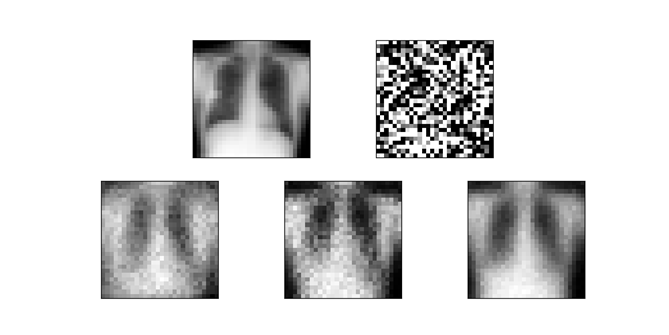
\includegraphics[width=0.4\textwidth]{foto/gaussian_lungs.png}
  \caption{On top, the original image and the image with Gaussian noise. On the bottom, starting from the left, the reconstruction of the image using PCA, fully connected DAE and convolutional DAE}
  \label{fig:gaussian_lungs}
\end{figure}

As expected, PCA performs the poorest, resulting in reconstructions with noticeable distortions. In contrast, the CNN-DAE delivers the most accurate and visually clear reconstruction. To support this qualitative assessment, we conducted a quantitative analysis by 
evaluating the MSE for the three methods while varying the latent dimension (for DAEs) and the number of principal components (for PCA). This approach allowed us to compare their performance and identify the optimal hyperparameters for each method.
Figure \ref{fig:MSE_gaussian} reveals that PCA consistently exhibits a higher error 
compared to the 

\begin{figure}[h]
  \centering
  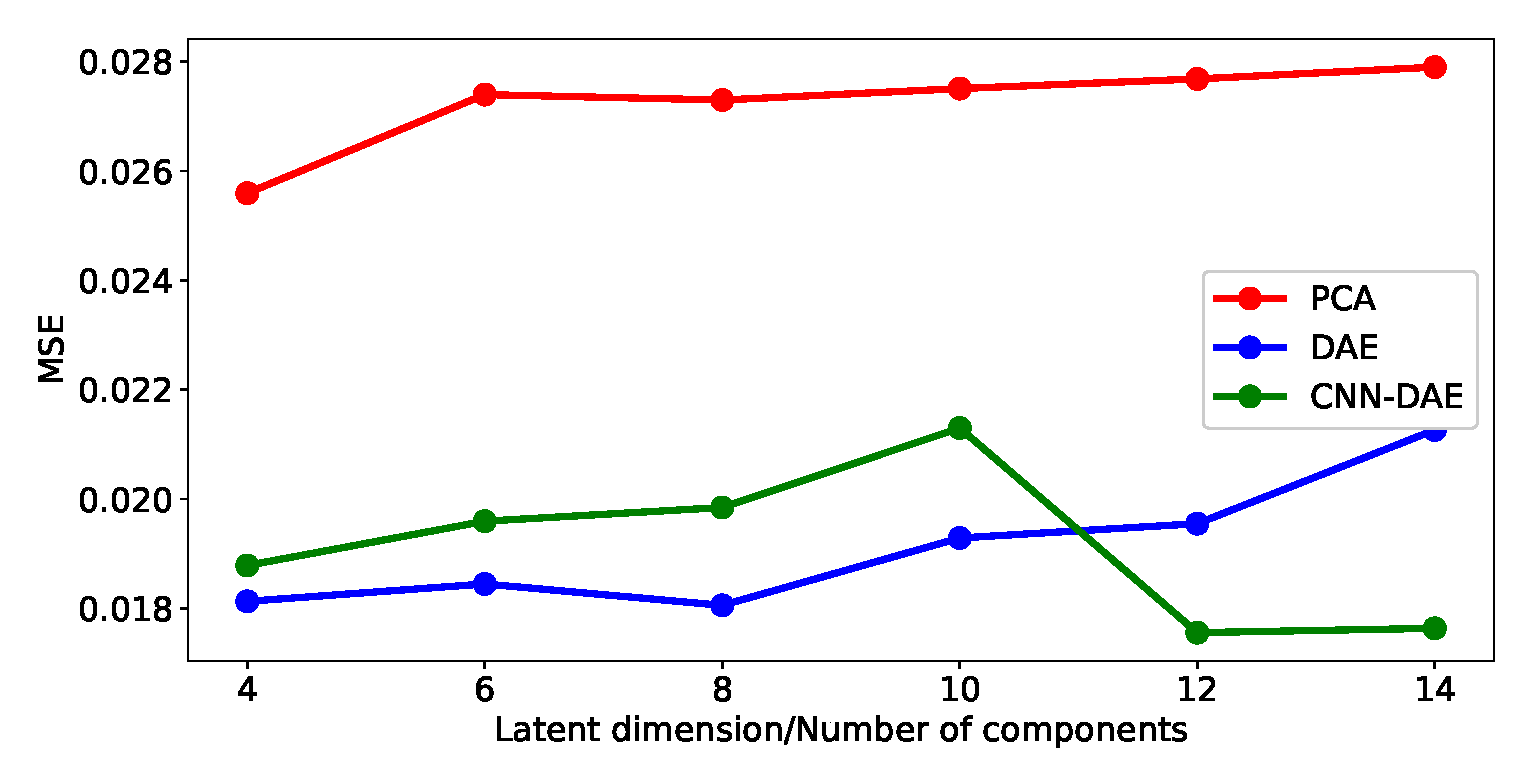
\includegraphics[width=0.5\textwidth]{foto/validation_gaussian.eps}
  \caption{MSE for PCA, DAE and CNN-DAE with Gaussian noise, varying the latent space size/number of principal components}
  \label{fig:MSE_gaussian}
\end{figure}

\noindent DAEs. Among the DAEs, both methods display a similar trend, but the CNN-DAE outperforms the fully connected DAE in higher dimensions, maintaining a lower error and avoiding the overfitting observed in the latter.\\

When analyzing the effects of Low Frequency noise, a distinct pattern emerges. This type of noise introduces structured distortions into the image, as illustrated in Figure \ref{fig:low_lungs}. In this scenario, both PCA and the fully connected DAE face challenges in accurately reconstructing the image, often overfitting to the noise. In contrast, the CNN-DAE demonstrates its ability to preserve the underlying structure of the data, resulting in a much clearer and more faithful reconstruction.

\begin{figure}[h!]
  \centering
  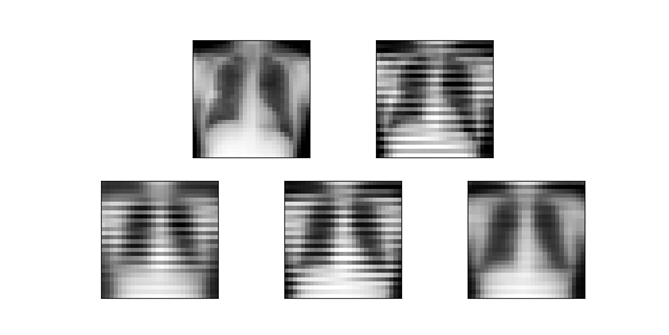
\includegraphics[width=0.4\textwidth]{foto/lowfreq_lungs.png}
  \caption{On top, the original image and the image with Low Frequency noise. On the bottom, starting from the left, the reconstruction of the image using PCA, fully connected DAE and convolutional DAE}
  \label{fig:low_lungs}
\end{figure}

The quantitative analysis in Figure \ref{fig:MSE_low_freq} reinforces this observation. PCA exhibits the highest error and a noticeable overfitting trend, which is similarly observed in the fully connected DAE. By contrast, the CNN-DAE consistently achieves lower error
rates and agains shows robustness to overfitting, even in the presence of structured noise. 

\begin{figure}[h!]
  \centering
  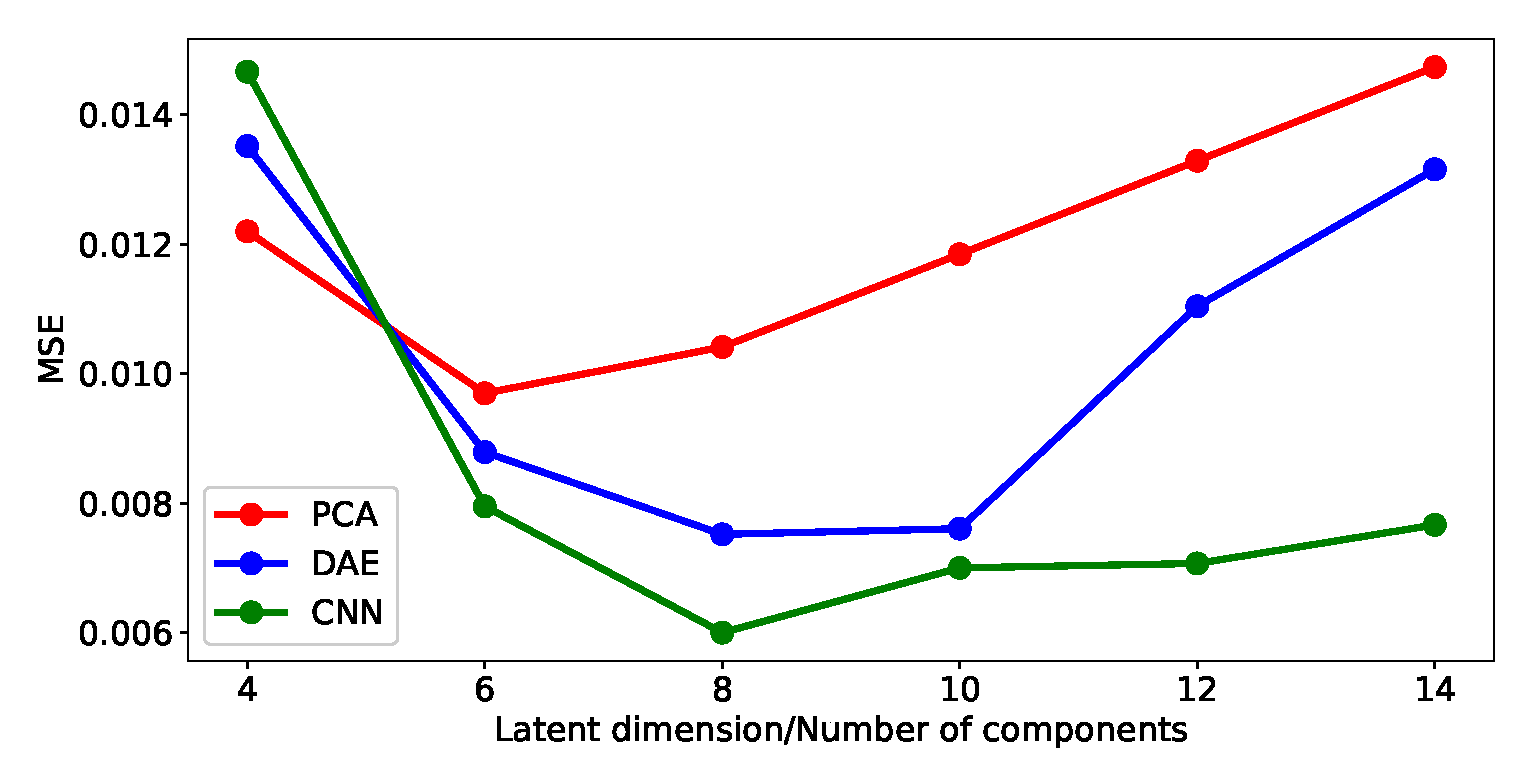
\includegraphics[width=0.5\textwidth]{foto/validation_low_freq.eps}
  \caption{MSE for PCA, DAE and CNN-DAE with Low Frequency noise, varying the latent space size/number of principal components}
  \label{fig:MSE_low_freq}
\end{figure}

In this scenario, the structured nature of the noise poses similar challenges for all three methods in capturing the underlying data patterns, without learning the perturbation. 
\quad 2) \textit{Computation Time}: Figure \ref{fig:runtime} illustrates the runtime for PCA, DAE, and CNN-DAE with Gaussian and Low Frequency noise, respectively. 

\begin{figure}[h!]
  \centering
  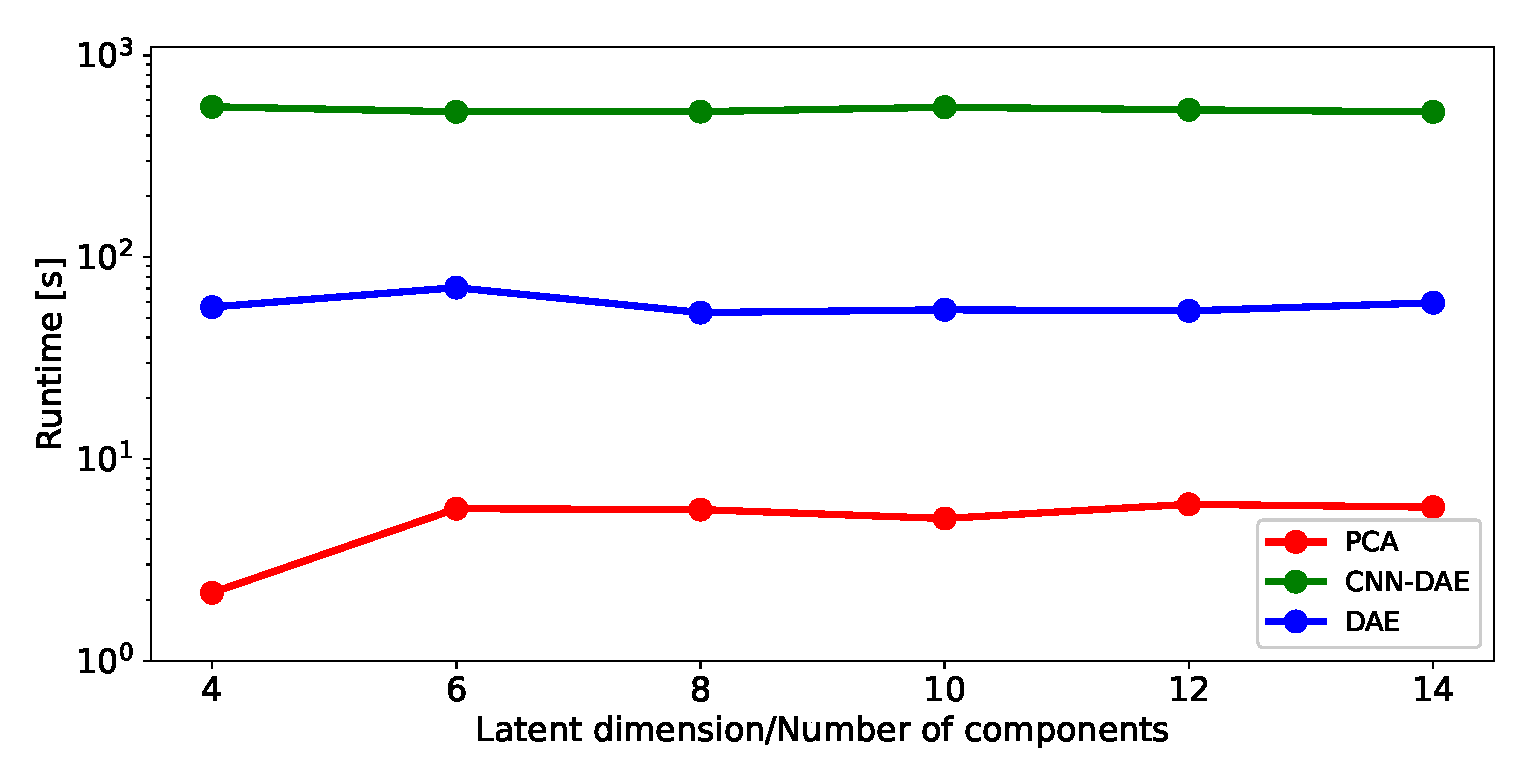
\includegraphics[width=0.5\textwidth]{foto/runtime_gaussian.eps}

  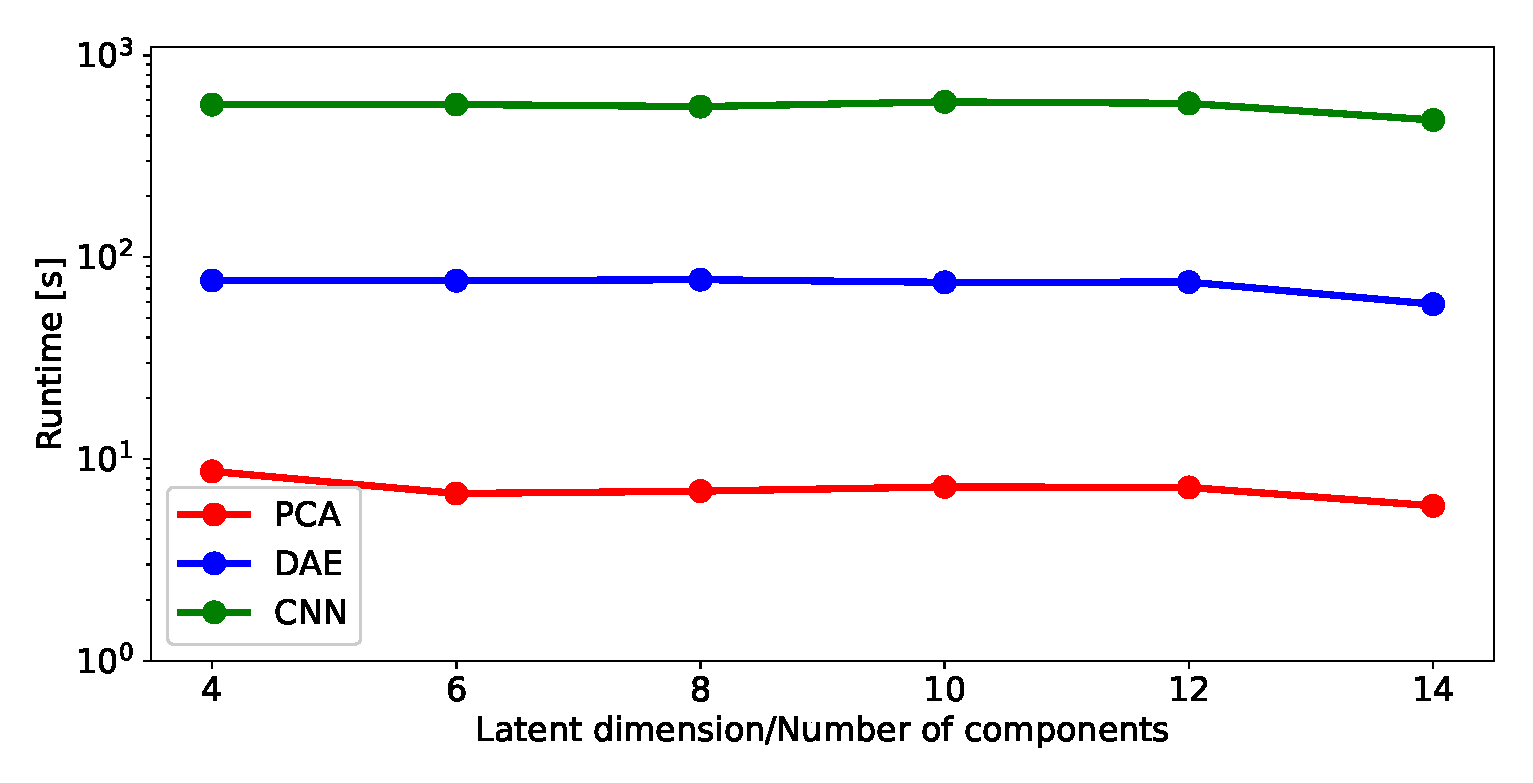
\includegraphics[width=0.5\textwidth]{foto/runtime_low_freq.eps}
  \caption{Runtime (in seconds) for PCA, DAE and CNN-DAE with Gaussian (top) and Low Frequency (bottom) noise, varying the latent space size/number of principal components}
  \label{fig:runtime}
\end{figure}

The computation time seems not to be correlated with the dimension of the latent space: this is explained by the fact that the increase in the number of weights connected to the latent layer is relatively small, compared to the total number of weights in the network. This is consistent with the architecture of the autoencoder, where the latent dimension is much smaller than in all the other layers. On the other hand, the computational cost varies a lot across the three methods. PCA is significantly faster than the fully connected DAE, which in turn are faster than the CNN. 
PCA is a relatively simple algorithm that mainly involves matrix multiplications and SVD calculation, resulting in a lower computational cost. On the other hand, neural networks solve complex optimization problems, 
which inherently require more computational resources. Among these, CNNs have the highest computational cost despite having a more sparse structure, as they involve additional processes like pooling and  convolution operations, which significantly increases the overall computational burden.


\section{Comparison between DAE and CNN-DAE}
As we can see from the simulation we conducted, the fully connected DAE and the convolutional DAE showed a significant difference in performance, with the latter outperforming the former 
in both types of noise. This result led us to analyze the reasons behind this difference, and we have identified the following considerations.

\subsection{Structure of Noise and Signal}
The type of noise present in the data plays a significant role in shaping how different models respond. When the noise is spatially correlated or structured, a high-capacity 
autoencoder may interpret these noise patterns as part of the signal and try to reconstruct them. This behavior can lead to overfitting, as the model captures 
the noise details rather than focusing on the underlying data structure. On the other hand, CNNs, due to their ability to detect local patterns and apply operations like pooling, have an edge when the noise is spatially incoherent. Therefore, in cases of random noise, CNNs generally perform better by generalizing well to the clean signal.

\subsection{Regularization}
CNNs inherently incorporate regularization due to their architecture. The use of shared weights in convolutional layers reduces the number of parameters, which helps control 
model complexity and prevent overfitting. This weight sharing ensures that the model does not learn redundant or irrelevant patterns in different parts of the input. 
Additionally, pooling operations, such as max-pooling or average-pooling, help reduce the spatial resolution of the data while retaining important features. 
These operations also filter out high-frequency variations, which often correspond to noise, thus preventing the model from memorizing random fluctuations in 
the input data. In essence, the design of CNNs offers built-in regularization, making them less prone to overfitting compared to models without such constraints, 
like fully connected autoencoders.

\subsection{Challenges in Noise-to-Noise Training}
In noise-to-noise training, the model learns to reconstruct a clean signal from noisy inputs using noisy targets. This approach presents challenges for different 
models. A classic autoencoder might struggle in this scenario, as it does not have a built-in mechanism to distinguish signal from noise. Instead, it could learn 
to map noise in the input to noise in the target, which leads to poor generalization. CNNs, however, have a natural advantage in this setting. Their ability to 
capture local features and filter out irrelevant variations through convolutions and pooling operations allows them to focus on the underlying structure of the 
signal, even when both the input and target are noisy. This ability to generalize well in the presence of noise makes CNNs more effective in noise-to-noise training 
tasks.

\subsection{Inductive Bias}
One key difference between classic autoencoders and CNNs is the presence of inductive bias. autoencoders typically do not come with any strong 
assumptions about the structure of the data. They are flexible models that can fit a wide variety of data patterns, but this flexibility also means 
that they can capture irrelevant details, such as noise, that are not crucial to the underlying signal. In contrast, CNNs are specifically designed 
to work with data that exhibits local and hierarchical structures, such as images. This inductive bias towards local feature extraction helps CNNs 
focus on the most significant patterns in the data while ignoring irrelevant noise. As a result, CNNs are less likely to overfit in cases where the 
data contains structured or unstructured noise.

\subsection{Overparameterization}
When working with small datasets or datasets with a low signal-to-noise ratio, overfitting becomes a serious concern. In such cases, 
models with excessive parameters, like autoencoders with many hidden units or deep architectures, are more likely to memorize the 
training data, including the noise, rather than generalizing to the underlying signal. This overparameterization problem is less 
pronounced in CNNs because of the limited number of parameters due to weight sharing in convolutional layers. 

\section{Conclusion}
This report presents a comparison between PCA and autoencoders for a denoising task. We found that while PCA is a simple and fast method that offers interpretability 
through low-rank approximation, it struggles to capture the underlying structure of the data as effectively as autoencoders. In particular, the Convolutional 
DAE outperformed the Fully Connected DAE, especially when the noise follows a structured pattern, demonstrating better generalization and avoiding overfitting, 
although it comes at a higher computational cost.\\
For future research, improving the performance of the fully connected DAE could be a valuable direction. Potential strategies include adding regularization techniques such as dropout or 
L1/L2 weight decay, reducing model complexity by using fewer hidden units or layers, and leveraging data augmentation to increase dataset variety. These approaches could help the model generalize better and minimize the risk of overfitting.\\
Overall, the CNN-DAE appears to be the most reliable choice for the denoising task, providing the best results. However, PCA remains a valid option when computational cost is a concern and the data is not excessively noisy or structured.


\begin{thebibliography}{9}
\bibitem{pca}
Jolliffe, I. T. (2002). Principal Component Analysis. Springer Series in Statistics.

\bibitem{autoencoders}
Goodfellow, I., Bengio, Y., Courville, A. (2016). Deep Learning. MIT Press.
\end{thebibliography}

\end{document}